\section{Launcher requirements}
\qquad \underline{By} : Alexis\\

From our initial requirements we set to stay within certain margins of size and mass. These two parameters create constraint for the launch. 
Indeed, we have to analyze the different launcher on the market and their capabilities. 
Thus, we chose to stay within the capabilities of two of the most used actual launchers: Ariane 6.4 and Falcon 9. \\

These launchers have almost the same launch capability; the Falcon 9 can send $22.8$ t in LEO and Ariane 6.4 can send $21.6$ t to LEO.
The other important characteristic is the dimension of the fairing.
Here we have two different launchers with almost identical size; the Falcon 9 can carry a payload up to $11.4$ m long and $4.6$ m wide, whereas Ariane 6.4 can carry up to $18$ m long and $4.57$ m wide but as the Ariane's fairing is very elongated the true usable size will be more around $12$ m by $4.57$ m. \\

To allow us to correctly design our spacecraft we need to create a theoretical envelope based on these two launchers. For that we set the following dimension: a diameter of $4.5$ m and a total length of $11.4$ m. These dimensions are lower than the two launchers to unsure to have a safety margin.

\clearpage

To sum up, here is the 3 fairing we spoke about:

\begin{figure}[H]
    \centering
    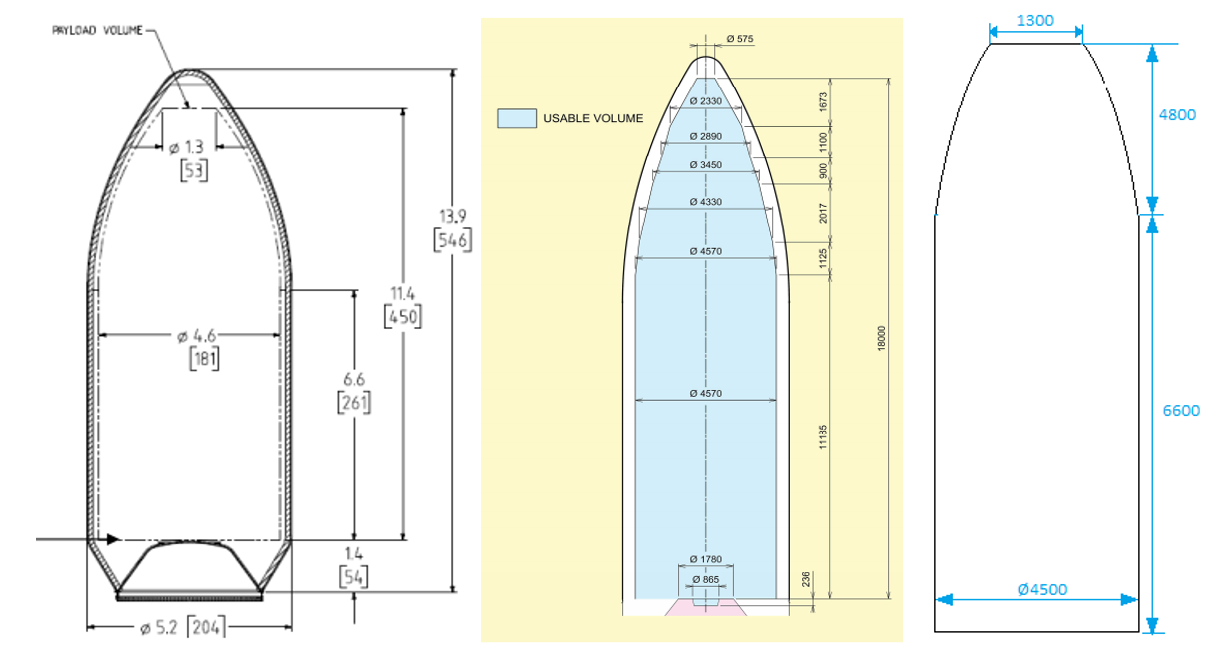
\includegraphics[width=\linewidth]{enveloppe}
    \caption{Falcon 9 - Ariane 6 - combined fairing}
    \label{fig:my_label}
\end{figure}

In case, during the design process, the spacecraft cannot stay behind the 22t to LEO launch capability of the Falcon 9, we plan to use the bigger Falcon Heavy which can send 60t to LEO. This launcher will be the last choice, we want at most to stay within our pre-requirement. \\

We first think to use the structure of our spacecraft, which is aerodynamic, as a fairing so we have less constraint on the size but as it has wings and tail it will generate a small lift but sufficient to destabilize the launcher and might cause a crash. So we decided to forget this idea and to stay within a classic fairing. \\

Through our project we are going to see if our requirements can meet our calculations and we will make a choice of launcher. 